% +------------------------------------------------------------------------+
% | CGAL Reference Manual:  Box_intersection_d/main.tex
% +------------------------------------------------------------------------+
% | Fast iso-box intersections
% |
% | 2003, 2004   Lutz Kettner, Andreas Meyer, Afra Zomorodian
% | 
\RCSdef{\BoxIntersectionRev}{$Id$}
\RCSdefDate{\BoxIntersectionDate}{$Date$}
% +------------------------------------------------------------------------+

\ccParDims
\ccUserChapter{Intersecting Sequences of dD Iso-oriented Boxes\label{chapterBoxIntersection}}
\ccChapterRelease{\BoxIntersectionRev. \ \BoxIntersectionDate}
\ccChapterAuthor{Lutz Kettner \and Andreas Meyer \and Afra Zomorodian}


\begin{ccPkgDescription}{3D Triangulations}
\ccPkgSummary{
This package  allows to build and handle
triangulations for point sets in three dimensions.
Any CGAL  triangulation covers the convex hull of its
vertices. Triangulations are build incrementally 
and can be modified by insertion or removal of vertices. 
They offer point location facilities.

The package provides plain triangulation (whose faces
depends on the  insertion order of the vertices) and
Delaunay triangulations.  Regular triangulations are
also provided for sets of weighted points.
Delaunay and regular
triangulations offer nearest neighbor queries
and primitives to build the dual Voronoi and power diagrams.}

%\ccPkgDependsOn{}
\ccPkgMaturity{Introduced in \cgal\ 3.1}

\end{ccPkgDescription}


\begin{ccTexOnly}
    \setlength{\unitlength}{1mm}
    \begin{picture}(0,0)(0.0,0.0)
      \put (90,20){
          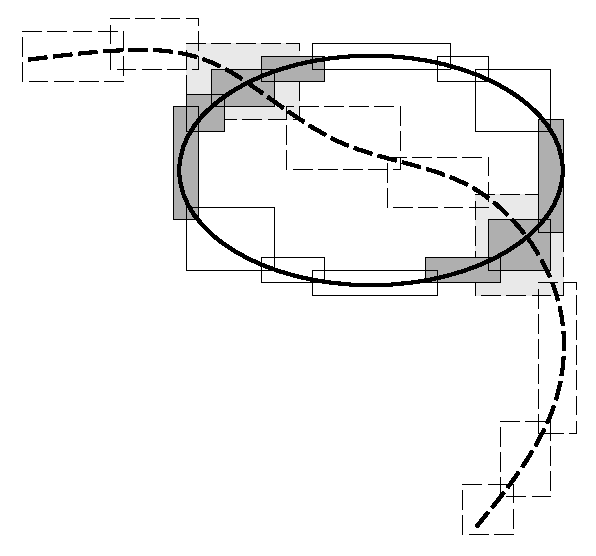
\includegraphics[width=70mm]{Box_intersection_d/fig/box_inters}
      }
    \end{picture}\vspace{-4mm}% compensate for some vspace added by picture
\end{ccTexOnly}

\minitoc

% +------------------------------------------------------------------------+
\section{Introduction}

Simple questions on geometric primitives, such as intersection and
distance computations, can themselves become quite expensive if the
primitives are not so simple anymore, for example, three-dimensional
triangles and facets of polyhedral surfaces. Thus algorithms operating
on these primitives tend to be slow in practice. A common (heuristic)
optimization approximates the geometric primitives with their
axis-aligned bounding boxes, runs a suitable modification of the
algorithm on the boxes, and whenever a pair of boxes has an
interesting interaction\footnote{Boxes represent volumes or point-sets. So, \textit{intersection} means intersection of the point-set enclosed by the box and not only intersection of the boundary, of course.}, only then the exact answer is computed on the
complicated geometric primitives contained in the boxes.

\begin{ccHtmlOnly}
    <CENTER>
        <img src="./fig/box_inters.gif" alt="Two intersecting curves with
        approximating boxes."><P>
    </CENTER>
\end{ccHtmlOnly}

We provide an efficient algorithm~\cite{cgal:ze-fsbi-02} for finding all
intersecting pairs for large numbers of iso-oriented boxes, i.e.,
typically these will be such bounding boxes of more complicated geometries.
One immediate application of this algorithm is the detection of all
intersections (and self-intersections) for polyhedral surfaces, i.e.,
applying the algorithm on a large set of triangles in space, we give
an example program later in this chapter. Not so obvious applications
are proximity queries and distance computations among such surfaces,
see Section~\ref{sec:box_inters_example_proximity} for an example
and~\cite{cgal:ze-fsbi-02} for more details.  

% +------------------------------------------------------------------------+
\section{Definition\label{sec:box-inters-def}}

A $d$-dimensional iso-oriented box is defined as the
Cartesian product of $d$ intervals. We call the
box \emph{half-open} if the $d$ intervals $\{ [lo_i,hi_i) \,|\, 0 \leq
i < d\}$ are half-open intervals, and we call the box \emph{closed} if
the $d$ intervals $\{ [lo_i,hi_i] \,|\, 0 \leq i < d\}$ are closed
intervals. Note that closed boxes support zero-width boxes and they
can intersect at their boundaries, while non-empty half-open boxes
always have a positive volume and they only intersect iff their
interiors overlap.  The distinction between closed and half-open boxes
does not require a different representation of boxes, just a different
interpretation when comparing boxes, which is selected with the two
possible values for the \ccc{topology} parameter:

\begin{itemize}
  \item \ccc{CGAL::Box_intersection_d::HALF_OPEN} and
  \item \ccc{CGAL::Box_intersection_d::CLOSED}.
\end{itemize}

The number type of the interval boundaries must be one of the built-in
types \texttt{int}, \texttt{unsigned int}, \texttt{double} or
\texttt{float}.

In addition, a box has an unique \ccc{id}-number. It is used to order
boxes consistently in each dimension even if boxes have identical
coordinates. In consequence, the algorithm guarantees that a pair of
intersecting boxes is reported only once. Note that boxes with equal
\ccc{id}-number are not reported since they obviously intersect trivially.

The box intersection algorithm comes in two flavors: One algorithm
works on a single sequence of boxes and computes all pairwise
intersections, which is called the \emph{complete\/} case, and used,
for example, in the self-intersection test. The other algorithm works
on two sequences of boxes and computes the pairwise intersections
between boxes from the first sequence with boxes from the second
sequence, which is called the \emph{bipartite\/} case. For each
pairwise intersection found a callback function is called with two
arguments; the first argument is a box from the first sequence and the
second argument a box from the second sequence. In the complete case,
the second argument is a box from an internal copy of the first
sequence.


% +------------------------------------------------------------------------+
\section{Software Design}

The box intersection algorithm is implemented as a family of generic
functions; the functions for the complete case accept one iterator
range, and the functions for the bipartite case accept two iterator
ranges. The callback function for reporting the intersecting pairs is
provided as a template parameter of the \ccc{BinaryFunction} concept.
The two principle function calls utilizing all default arguments look
as follows:

\ccInclude{CGAL/box_intersection_d.h}

\ccThree{void}{box_inter}{}
%\def\ccLongParamLayout{\ccTrue}
\ccGlobalFunction{template< class RandomAccessIterator, class Callback >
void box_intersection_d(
    RandomAccessIterator begin, RandomAccessIterator end,
    Callback callback);}

\ccGlobalFunction{template< class RandomAccessIterator1, 
                  class RandomAccessIterator2, 
                  class Callback >
void box_intersection_d(
    RandomAccessIterator1 begin1, RandomAccessIterator1 end1,
    RandomAccessIterator2 begin2, RandomAccessIterator2 end2,
    Callback callback);}


Additional parameters to the functions calls are a \emph{cutoff\/}
value to adjust performance trade-offs, and a \emph{topology\/} parameter
selecting between topologically closed boxes (the default) and
topologically half-open boxes.

The algorithm reorders the boxes in the course of the algorithm. Now,
depending on the size of a box it can be faster to copy the boxes, or
to work with pointers to boxes and copy only pointers. We offer
automatic support for both options. To simplify the description, let us
call the \ccc{value_type} of the iterator ranges \emph{box handle}.
The \emph{box handle\/} can either be our box type itself or a
pointer (or const pointer) to the box type; these choices represent
both options from above.

In general, the algorithms treat the box type as opaque type and just
assume that they are models of the \ccc{Assignable} concept, so that
the algorithms can modify the input sequences and reorder the boxes.
The access to the box dimension and box coordinates is mediated with a
traits class of the \ccc{BoxIntersectionTraits_d} concept. A default
traits class is provided that assumes that the box type is a model of
the \ccc{BoxIntersectionBox_d} concept and that the box handle, i.e.,
the iterators value type, is identical to the box type or a pointer
to the box type (see the previous paragraph for the value versus
pointer nature of the box handle).

Two implementations of iso-oriented boxes are provided;
\ccc{CGAL::Box_intersection_d::Box_d} as a plain box, and
\ccc{CGAL::Box_intersection_d::Box_with_handle_d} as a box plus a
handle that can be used to point to the full geometry that is
approximated by the box. Both implementations have template parameters
for the number type used for the interval bounds, for the fixed
dimension of the box, and for a policy class~\cite{cgal:a-mcdgp-01}
selecting among several solutions for providing the \ccc{id}-number.

The function signatures for the bipartite case look as follows. The 
signatures for the complete case with the \ccc{box_self_intersection_d}
function look the same except for the single iterator range.

\ccInclude{CGAL/box_intersection_d.h}

\ccThree{void}{box_inter}{}
%\def\ccLongParamLayout{\ccTrue}
\ccGlobalFunction{template< class RandomAccessIterator1, 
            class RandomAccessIterator2, 
            class Callback >
void box_intersection_d(
    RandomAccessIterator1 begin1, RandomAccessIterator1 end1,
    RandomAccessIterator2 begin2, RandomAccessIterator2 end2,
    Callback callback,
    std::ptrdiff_t cutoff = 10,
    Box_intersection_d::Topology topology = Box_intersection_d::CLOSED,
    Box_intersection_d::Setting  setting  = Box_intersection_d::BIPARTITE);}
 
\ccGlobalFunction{template< class RandomAccessIterator1,
            class RandomAccessIterator2,
            class Callback, class BoxTraits >
void box_intersection_d(
    RandomAccessIterator1 begin1, RandomAccessIterator1 end1,
    RandomAccessIterator2 begin2, RandomAccessIterator2 end2,
    Callback callback,
    BoxTraits box_traits,
    std::ptrdiff cutoff = 10,
    Box_intersection_d::Topology topology = Box_intersection_d::CLOSED,
    Box_intersection_d::Setting  setting  = Box_intersection_d::BIPARTITE);}


%\begin{ccAdvanced}
%  A more detailed interface is provided with the box predicate traits
%  class. It implements the various predicates used in the box
%  intersection algorithm. It is exchangeable and can be used by
%  experts to fine tune the comparisons performed in this algorithm,
%  e.g. utilizing machine instruction sets, see the
%  \ccc{BoxIntersectionPredicateTraits_d} concept in the reference
%  manual section for more details. Note that the generic default model
%  provided is fully functional and efficient in all cases, thus
%  usually there is no need to look at this predicate traits.
%\end{ccAdvanced}


% +------------------------------------------------------------------------+
\section{Minimal Example for Intersecting Boxes\label{sec:box-intersect-minimal}}

The box implementation provided with
\ccc{CGAL::Box_intersection_d::Box_d<double,2>} has a dedicated
constructor for the \cgal\ bounding box type \ccc{CGAL::Bbox_2}
(similar for dimension 3). We use this in our minimal example to
create easily nine two-dimensional \ccc{boxes} in a grid layout of $3
\times 3$ boxes. Additionally we pick the center box and the box in
the upper-right corner as our second box sequence \ccc{query}.

The default policy of the box type implements the \ccc{id}-number with
an explicit counter in the boxes, which is the default choice since it
always works, but it costs space that could potentially be avoided,
see the example in the next section. We use the \ccc{id}-number in our
callback function to report the result of the intersection algorithm.
The result will be that the first \ccc{query} box intersects all nine
\ccc{boxes} and the second \ccc{query} box intersects the four boxes
in the upper-right quadrant. See Section~\ref{sec:box-inters-params}
for the change of the \ccc{topology} parameter and its effect.

\ccIncludeExampleCode{Box_intersection_d/minimal.cpp}


% +------------------------------------------------------------------------+
\section{Example for Finding Intersecting 3D Triangles}

The conventional application of the axis-aligned box intersection
algorithm will start from complex geometry, here 3D triangles,
approximate them with their bounding box, compute the intersecting
pairs of boxes, and check only for those if the original triangles
intersect as well.

We start in the \ccc{main} function and create ten triangles with
endpoints chosen randomly in a cube $[-1,+1)^3$. We store the
triangles in a vector called \ccc{triangles}.

Next we create a vector for the bounding boxes of the triangles called
\ccc{boxes}. For the boxes we choose the type
\ccc{Box_with_handle_d<double,3,Iterator>} that works nicely together
with the \cgal\ bounding boxes of type \ccc{CGAL::Bbox_3}. In
addition, each box stores the iterator to the corresponding triangle.

The default policy of this box type uses for the \ccc{id}-number the 
address of the value of the iterator, i.e., the address of the
triangle. This is a good choice that works correctly iff the boxes
have unique iterators, i.e., there is a one-to-one mapping between
boxes and approximated geometry, which is the case here. It saves us
the extra space that was needed for the explicit \ccc{id}-number in
the previous example.

We run the self intersection algorithm with the \ccc{report_inters}
function as callback. This callback reports the intersecting boxes. It
uses the \ccc{handle} and the global \ccc{triangles} vector to
calculate the triangle numbers. Then it checks the triangles
themselves for intersection and reports if not only the boxes but also
the triangles intersect. We take some precautions before the
intersection test in order to avoid problems, although unlikely, with
degenerate triangles that we might have created with the random
process.

This example can be easily extended to test polyhedral surfaces of the
\ccc{Polyhedron_3} class for (self-) intersections. The main
difference are the numerous cases of incidences between triangles in
the polyhedral surface that should not be reported as intersections,
see the \texttt{examples/Polyhedron/polyhedron\_self\_intersection.cpp}
example program in the \cgal\ distribution. 

\ccIncludeExampleCode{Box_intersection_d/triangle_self_intersect.cpp}


% +------------------------------------------------------------------------+
\section{Example for Using Pointers to Boxes}

We modify the previous example, finding intersecting 3D triangles,
and add an additional vector \ccc{ptr} that stores pointers to the bounding
boxes, so that the intersection algorithm will work on a sequence of
pointers and not on a sequence of boxes. The change just affects the
preparation of the additional vector and the call of the box intersection
function. The box intersection function (actually its default traits
class) detects automatically that the value type of the iterators is a
pointer type and not a class type.

\begin{ccExampleCode}
    // Create the corresponding vector of pointers to bounding boxes
    std::vector<Box *> ptr;
    for ( std::vector<Box>::iterator i = boxes.begin(); i != boxes.end(); ++i)
        ptr.push_back( &*i);
    
    // Run the self intersection algorithm with all defaults on the 
    // indirect pointers to bounding boxes. Avoids copying the boxes.
    CGAL::box_self_intersection_d( ptr.begin(), ptr.end(), report_inters);
\end{ccExampleCode}

In addition, the callback function \ccc{report_inters} needs to be
changed to work with pointers to boxes. The full example program looks
as follows:

\ccIncludeExampleCode{Box_intersection_d/triangle_self_intersect_pointers.cpp}

A note on performance: The algorithm sorts and partitions the input
sequences. It is clearly costly to copy a large box compared to a
simple pointer. However, the algorithm benefits from memory locality
in the later stages when it copies the boxes, while the pointers would
refer to boxes that become wildly scattered in memory.  These two
effects, copying costs and memory locality, counteract each other. For
small box sizes, i.e., small dimension, memory locality wins and one
should work with boxes, while for larger box sizes one should work
with pointers. The exact threshold depends on the memory hierarchy
(caching) of the hardware platform and the size of the boxes, most
notably the type used to represent the box coordinates. A concrete
example; on a laptop with an Intel Mobile Pentium4 running at 1.80GHz
with 512KB cache and 254MB main memory under Linux this version with
pointers was 20\% faster than the version above that copies the boxes
for 10000 boxes, but the picture reversed for 100000 boxes, where the
version above that copies the boxes becomes 300\% faster.

Note that switching to the built-in type \ccc{float} is supported by
the box intersection algorithm, but the interfacing with the \cgal\ 
bounding box \ccc{CGAL::Bbox_3} would not be that easy. In particular,
just converting from the \ccc{double} to the \ccc{float}
representation incurs rounding that needs to be controlled properly,
otherwise the box might shrink and one might miss intersections.


% +------------------------------------------------------------------------+
\section{Example Using the \textit{topology} and the \textit{cutoff} 
Parameters\label{sec:box-inters-params}}

Boxes can be interpreted by the box intersection algorithm as closed
or as half-open boxes, see also Section~\ref{sec:box-inters-def}.  Closed
boxes support zero-width boxes and they can intersect at their
boundaries, while half-open boxes always have a positive volume and
they only intersect iff their interiors overlap.  The choice between
closed or half-open boxes is selected with the \ccc{topology}
parameter and its two values:

\begin{itemize}
  \item \ccc{CGAL::Box_intersection_d::HALF_OPEN} and
  \item \ccc{CGAL::Box_intersection_d::CLOSED}.
\end{itemize}

The example program uses a two-dimensional box with \ccc{int}
coordinates and \ccc{id}-numbers that are by default explicitly
stored. We create the same boxes as in the minimal example in
Section~\ref{sec:box-intersect-minimal}. We create a $3 \times 3$ grid
of \ccc{boxes}, and two boxes for the \ccc{query} sequence, namely the
box at the center and the box from the upper-right corner of the grid.

We write a more involved callback function object \ccc{Report} that
stores an output iterator and writes the \ccc{id}-number of the 
box in the first argument to the output iterator. We also provide a
small helper function \ccc{report} that simplifies the use of the function
object.

We call the box intersection algorithm twice; once for the default
\ccc{topology}, which is the closed box topology, and once for the
half-open box topology. We sort the resulting output for better
readability and verify its correctness with the \ccc{check1} and
\ccc{check2} data.  For the closed box topology, the center box in
\ccc{query} intersects all \ccc{boxes}, and the upper-right box in
\ccc{query} intersects the four boxes of the upper-right quadrant in
\ccc{boxes}. Almost all intersections are with the box boundaries,
thus, for the half-open topology only one intersection remains per
\ccc{query} box, namely its corresponding box in \ccc{boxes}. So, the
output of the algorithm will be:

\begin{verbatim}
    0 1 2 3 4 4 5 5 6 7 7 8 8 
    4 8 
\end{verbatim}

For the second box intersection function call we have to specify the
\ccc{cutoff} parameter explicitly. See the
Section~\ref{sec:box-inters-performance} below for a detailed
discussion.

\ccIncludeExampleCode{Box_intersection_d/box_grid.cpp}


% +------------------------------------------------------------------------+
\section{Runtime Performance\label{sec:box-inters-performance}}

The implemented algorithm is described in~\cite{cgal:ze-fsbi-02} as
version two.  Its performance depends on a \ccc{cutoff} parameter.
When the size of both iterator ranges drops below the \ccc{cutoff}
parameter the function switches from the streamed segment-tree
algorithm to the two-way-scan algorithm, see~\cite{cgal:ze-fsbi-02}
for the details.

The streamed segment-tree algorithm needs $O(n \log^d (n) + k)$
worst-case running time and $O(n)$ space, where $n$ is the number of
boxes in both input sequences, $d$ the (constant) dimension of the
boxes, and $k$ the output complexity, i.e., the number of pairwise
intersections of the boxes. The two-way-scan algorithm needs $O(n \log
(n) + l)$ worst-case running time and $O(n)$ space, where $l$ is the
number of pairwise overlapping intervals in one dimensions (the
dimension where the algorithm is used instead of the segment tree).
Note that $l$ is not necessarily related to $k$ and using the
two-way-scan algorithm is a heuristic.

Unfortunately, we have no general method to automatically determine an
optimal cutoff parameter, since it depends on the used hardware, the
runtime ratio between callback runtime and segment-tree runtime, and
of course the number of boxes to be checked and their distribution. In
cases where the callback runtime is dominant, it may be best to make
the threshold parameter small. Otherwise a \ccc{cutoff}$=\sqrt{n}$ can
lead to acceptable results. For well distributed boxes the original
paper~\cite{cgal:ze-fsbi-02} gives optimal cutoffs in the thousands.
Anyway, for optimal runtime some experiments to compare different
cutoff parameters are recommended.

To demonstrate that box intersection can be done quite fast, different
box sequences are intersected in the range between 4 and 800000 boxes
total.  We use three-dimensional default boxes of closed topology with
\ccc{float} coordinates and without additional data fields.  The
algorithm works directly on the boxes, not on pointer to boxes. Each
box intersection is reported to an empty dummy callback.

For each box set, a near-optimal cutoff parameter is determined using
an adaptive approximation. The runtime required for streaming is
compared against usual scanning.  Results on a Xeon 2.4GHz with 4GB
main memory can be seen in Figure \ref{fig_benchmark}. For a small
number of boxes, pure scanning is still faster than streaming with
optimal cutoff, which would just delegate the box sets to the scanning
algorithm. As there are more and more boxes, the overhead becomes less
important. 

\begin{figure}[htbp]
\begin{ccTexOnly}
\begin{center}
  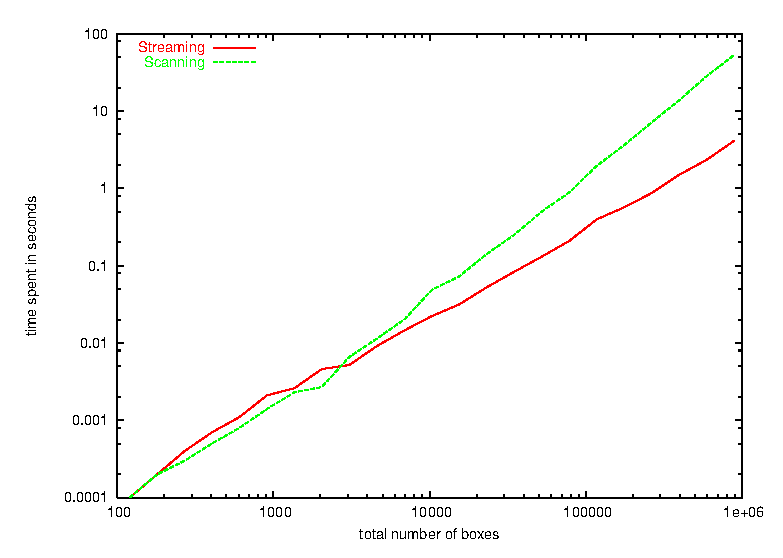
\includegraphics[width=0.7\textwidth]{Box_intersection_d/fig/benchmark}
\end{center}
\end{ccTexOnly}
\begin{ccHtmlOnly}
<center>
\end{ccHtmlOnly}

\begin{ccHtmlOnly}
<img border="0" src="./fig/benchmark.gif" align="center" alt="benchmark plot">
</center>
\end{ccHtmlOnly}

  \caption{Runtime comparison between the scanning and the streaming algorithm.
  \label{fig_benchmark}}
\end{figure}

% +------------------------------------------------------------------------+
\section{Example Using a Custom Box Implementation}

The example in the previous Section~\ref{sec:box-inters-params} uses
an array to provide the coordinates and then creates another array for
the boxes. In the following example we write our own box class
\ccc{Box} that we can initialize directly with the four coordinates and
create the array of boxes directly. We also omit the explicitly stored
\ccc{id}-number and use the address of the box itself as
\ccc{id}-number. This works only if the boxes do not change their
position, i.e., we work with pointers to the boxes in the intersection
algorithm.

We follow with our own box class \ccc{Box} the
\ccc{BoxIntersectionBox_d} concept, which allows us to reuse the
default traits implementation, i.e., we can use the same default
function call to compute all intersections. See the example in the
next section for a self-written traits class. So, in principle, the
remainder of the example stays the same and we omit the part from the
previous example for brevity that illustrates the half-open box topology.

The requirements for the box implementation are best studied on
page~\pageref{ccRef_BoxIntersectionBox_d} in the Reference Manual. In a
nutshell, we have to define the type \ccc{NT} for the box coordinates
and the type \ccc{ID} for the \ccc{id}-number. Member functions
give access to the coordinates and the \ccc{id}-number. A static
member function returns the dimension.

\ccIncludeExampleCode{Box_intersection_d/custom_box_grid.cpp}


% +------------------------------------------------------------------------+
\section{Example for Point Proximity Search with a Custom Traits Class\label{sec:box_inters_example_proximity}}

Given a set of 3D points, we want to find all pairs of points that are
less than a certain distance apart. We use the box intersection
algorithm to find good candidates, namely those that are less than
this specified distance apart in the $L_\infty$ norm, which is a good
approximation of the Euclidean norm.

We use an unusual representation for the box, namely pointers to the 3D points
themselves. We implement a special box traits class that interprets
the point as a box of the dimensions $[-$\ccc{eps}$,+$\ccc{eps}$]^3$
centered at this point. The value for \ccc{eps} is half the specified distance
from above, i.e., points are reported if their distance is smaller
than \ccc{2*eps}.

The requirements for the box traits class are best studied on
page~\pageref{ccRef_BoxIntersectionTraits_d} in the Reference Manual. In a
nutshell, we have to define the type \ccc{NT} for the box coordinates,
the type \ccc{ID} for the \ccc{id}-number, and the type \ccc{Box_parameter}
similar to the box handle, here \ccc{Point_3*} since we work with the pointers.
All member functions in the traits class are static. Two functions give
access to the max and min coordinates that we compute from the point
coordinates plus or minus the \ccc{eps} value, respectively. For the
\ccc{id}-number function the address of the point itself is
sufficient, since the points stay stable. Another function
returns the dimension.

The \ccc{report} callback function computes than the Euclidean
distance and prints a message for points that are close enough.

Note that we need to reserve sufficient space in the \ccc{points}
vector to avoid reallocations while we create the \ccc{points} vector
and the \ccc{boxes} vector in parallel, since otherwise the
\ccc{points} vector might reallocate and invalidate all pointers
stored in the \ccc{boxes} so far.

\ccIncludeExampleCode{Box_intersection_d/proximity_custom_box_traits.cpp}

% +------------------------------------------------------------------------+
\section{Design and Implementation History}

Lutz Kettner and Andreas Meyer implemented the algorithms starting
from the publication~\cite{cgal:ze-fsbi-02}. We had access to the
original C implementation of Afra Zomorodian, which helped clarifying
some questions, and we are grateful to the help of Afra Zomorodian in
answering our questions during his visit. We thank Steve Robbins for
an excellent review for this package. Steve Robbins provided an
independent and earlier implementation of this algorithm,
however, we learned too late about this implementation.


%% EOF %%
